% Document/LinearAlgebra/VectorSpaces/Foundations/LinearIndependence.tex
% Section: Linear Independence

\newpage
\section{Linear Independence}

\begin{remark}[Intuition]
    Not all vectors contribute equally to a span. Some vectors are ``redundant''---they can be
    expressed in terms of others. Linear independence captures the notion that each vector
    in a set genuinely adds new directions.
\end{remark}

\begin{example}[Linear Independence and Dependence]\label{ex:lin-indep-dep}
    Consider the following examples in $\bb{R}^2$ and $\bb{R}^3$:

    \textbf{Linearly independent sets}:
    \begin{itemize}
        \item $\{(1, 0), (0, 1)\}$ in $\bb{R}^2$
        \item $\{1, X, X^2\}$ in $K[X]$
        \item $\{e_1, e_2, e_3\}$ (standard basis) in $\bb{R}^3$
    \end{itemize}

    \textbf{Linearly dependent sets}:
    \begin{itemize}
        \item $\{(1, 0), (2, 0)\}$ in $\bb{R}^2$ (one is a scalar multiple of the other)
        \item $\{(1, 0, 0), (0, 1, 0), (1, 1, 0)\}$ in $\bb{R}^3$ (the third is the sum of the first two)
    \end{itemize}

    \begin{center}
    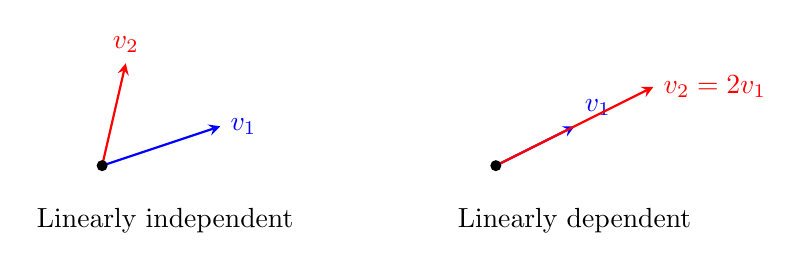
\begin{tikzpicture}[scale=1.0, >=stealth]
        % Linearly independent
        \begin{scope}
            \draw[->, thick, blue] (0,0) -- (1.5,0.5) node[right] {$v_1$};
            \draw[->, thick, red] (0,0) -- (0.3,1.3) node[above] {$v_2$};
            \fill (0,0) circle (2pt);
            \node at (0.8,-0.7) {Linearly independent};
        \end{scope}

        % Linearly dependent
        \begin{scope}[xshift=5cm]
            \draw[->, thick, blue] (0,0) -- (1,0.5) node[above right] {$v_1$};
            \draw[->, thick, red] (0,0) -- (2,1) node[right] {$v_2 = 2v_1$};
            \fill (0,0) circle (2pt);
            \node at (1,-0.7) {Linearly dependent};
        \end{scope}
    \end{tikzpicture}
    \end{center}
\end{example}

\begin{example}[Linear Independence in $\bb{R}^3$]\label{ex:lin-indep-R3}
    Consider the following cases in $\bb{R}^3$:

    \textbf{Independent (3 vectors spanning $\bb{R}^3$)}:
    \begin{itemize}
        \item $\{e_1, e_2, e_3\} = \{(1,0,0), (0,1,0), (0,0,1)\}$ --- the standard basis
        \item $\{(1,1,0), (1,0,1), (0,1,1)\}$ --- three non-coplanar vectors
    \end{itemize}

    \textbf{Dependent (more than $\dim = 3$ vectors)}:
    \begin{itemize}
        \item $\{e_1, e_2, e_3, (1,1,1)\}$ --- any 4 vectors in $\bb{R}^3$ are dependent
    \end{itemize}

    \textbf{Dependent (coplanar vectors)}:
    \begin{itemize}
        \item $\{(1,0,0), (0,1,0), (1,1,0)\}$ --- three vectors in the $xy$-plane satisfy $(1,1,0) = (1,0,0) + (0,1,0)$
    \end{itemize}

    \begin{center}
    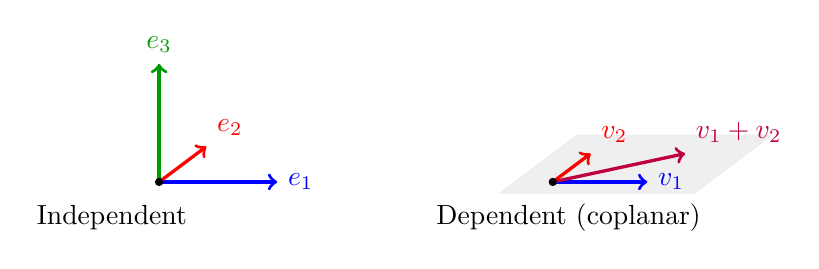
\begin{tikzpicture}[scale=1.0,
        x={(1cm,0cm)},
        y={(0.4cm,0.3cm)},
        z={(0cm,1cm)}]

        % Independent: 3 axes
        \begin{scope}
            \draw[->, very thick, blue] (0,0,0) -- (1.5,0,0) node[right] {$e_1$};
            \draw[->, very thick, red] (0,0,0) -- (0,1.5,0) node[above right] {$e_2$};
            \draw[->, very thick, green!60!black] (0,0,0) -- (0,0,1.5) node[above] {$e_3$};
            \fill (0,0,0) circle (1.5pt);
            \node at (0,-1.5,0) {Independent};
        \end{scope}

        % Dependent: coplanar
        \begin{scope}[xshift=5cm]
            \fill[gray!20, opacity=0.6] (-0.5,-0.5,0) -- (2,-0.5,0) -- (2,2,0) -- (-0.5,2,0) -- cycle;
            \draw[->, very thick, blue] (0,0,0) -- (1.2,0,0) node[right] {$v_1$};
            \draw[->, very thick, red] (0,0,0) -- (0,1.2,0) node[above right] {$v_2$};
            \draw[->, very thick, purple] (0,0,0) -- (1.2,1.2,0) node[above right] {$v_1 + v_2$};
            \fill (0,0,0) circle (1.5pt);
            \node at (0.8,-1.5,0) {Dependent (coplanar)};
        \end{scope}
    \end{tikzpicture}
    \end{center}
\end{example}

\begin{intuition}[Linear Dependence on a Set]
    Let $S \subseteq V$ and $v \in S$. Intuitively, we say $v$ is \textbf{linearly dependent on} $S \setminus \{v\}$
    if $v \in \Span[K]{S \setminus \{v\}}$---that is, $v$ can be expressed as a linear combination of the
    other vectors in $S$. Linear dependence is formally defined below as ``not linearly independent.''
\end{intuition}

\begin{example}[Dependence Examples]\label{ex:dependence}
    In $\bb{R}^3$ with standard basis $\{e_1, e_2, e_3\}$:
    \begin{itemize}
        \item $(1, 2, 3)$ is linearly dependent on $\{e_1, e_2, e_3\}$ because
              $(1, 2, 3) = 1 \cdot e_1 + 2 \cdot e_2 + 3 \cdot e_3 \in \Span[\bb{R}]{\{e_1, e_2, e_3\}}$.
        \item $e_1$ is linearly \emph{independent} of $\{e_2, e_3\}$ because
              $e_1 = (1, 0, 0) \notin \Span[\bb{R}]{\{e_2, e_3\}} = \Set{(0, y, z) \mid y, z \in \bb{R}}$.
    \end{itemize}
\end{example}

\begin{definition}[Unique Representation]\label{def:unique-rep}
    Let $L \subseteq V$. A vector $v \in V$ has \textbf{unique representation} in terms of $L$ if
    there exists a \textbf{unique} finite subset $F \subseteq L$ and \textbf{unique nonzero} scalars
    $(a_\ell)_{\ell \in F}$ such that
    \[
        v = \sum_{\ell \in F} a_\ell \ell
    \]
    The requirement that scalars be nonzero ensures uniqueness: otherwise we could add
    $0 \cdot w$ for any $w \in L \setminus F$.
\end{definition}

\begin{theorem}[Characterizations of Linear Independence]\label{thm:lin-indep-equiv}
    Let $L \subseteq V$. The following are equivalent:
    \begin{enumerate}
        \item[(i)] $\Forall :{v \in L}{\Span[K]{\{v\}} \Intersect \Span[K]{L \setminus \{v\}} = \{0\}}$
        \item[(i')] $\Forall :{v \in L}{\Span[K]{L \setminus \{v\}} \subsetneq \Span[K]{L}}$
        \item[(ii)] Every $v \in \Span[K]{L}$ has unique representation in terms of $L$
        \item[(iii)] Some $v \in \Span[K]{L}$ has unique representation
        \item[(iv)] $0$ has unique representation (i.e., if $0 = \sum_{i=1}^n a_i \ell_i$ with
              $\ell_i \in L$ distinct and $a_i \neq 0$, then $n = 0$)
    \end{enumerate}
\end{theorem}

\begin{proof}
    \textbf{(i') $\Leftrightarrow$ (i)}:
    We have $\Span[K]{\{v\}} \Intersect \Span[K]{L \setminus \{v\}} = \{0\}$ iff $v \notin \Span[K]{L \setminus \{v\}}$
    (since $\Span[K]{\{v\}} = \Set{\lambda v \mid \lambda \in K}$).
    This is equivalent to $\Span[K]{L \setminus \{v\}} \neq \Span[K]{L}$
    (since $\Span[K]{L} = \Span[K]{(L \setminus \{v\}) \Union \{v\}}$).

    \textbf{(ii) $\Rightarrow$ (iii)}:
    Trivial.

    \textbf{(iii) $\Rightarrow$ (iv)}:
    Suppose $v \in \Span[K]{L}$ has unique representation $v = \sum_{\ell \in F} a_\ell \ell$.
    If $0 = \sum_{\ell \in G} b_\ell \ell$ with $b_\ell \neq 0$, then
    \[
        v = v + 0 = \sum_{\ell \in F} a_\ell \ell + \sum_{\ell \in G} b_\ell \ell
    \]
    For this to be the unique representation of $v$, we need $G = \emptyset$.

    \textbf{(iv) $\Rightarrow$ (ii)}:
    Suppose $v = \sum_{\ell \in F} a_\ell \ell = \sum_{\ell \in G} b_\ell \ell$ are two representations
    (with nonzero coefficients). Then
    \[
        0 = \sum_{\ell \in F} a_\ell \ell - \sum_{\ell \in G} b_\ell \ell
    \]
    By (iv), all coefficients must be zero after combining like terms.
    This means $F = G$ and $a_\ell = b_\ell$ for all $\ell \in F$.

    \textbf{(i) $\Rightarrow$ (iv)} (requires field axioms):
    Suppose $0 = \sum_{i=1}^n a_i \ell_i$ with $a_i \neq 0$ and $n \geq 1$.
    Then $\ell_1 = -\frac{1}{a_1}\sum_{i=2}^n a_i \ell_i \in \Span[K]{L \setminus \{\ell_1\}}$,
    contradicting (i').

    \textbf{(iv) $\Rightarrow$ (i)} (does not require field axioms):
    Suppose $v \in \Span[K]{\{v\}} \Intersect \Span[K]{L \setminus \{v\}}$ with $v \neq 0$.
    Then $v = \lambda v$ for some $\lambda \in K$ and $v = \sum_{\ell \neq v} b_\ell \ell$.
    Thus $0 = (\lambda - 1)v - \sum_{\ell \neq v} b_\ell \ell$.
    If $v \notin \{\ell_1, \ldots, \ell_n\}$ (the summands), this is a nontrivial relation, contradicting (iv).
\end{proof}

\begin{definition}[Linearly Independent Set]\label{def:lin-indep}
    A subset $L \subseteq V$ is \textbf{linearly independent} if it satisfies any (hence all) of
    the equivalent conditions in Theorem~\ref{thm:lin-indep-equiv}.

    A set that is not linearly independent is called \textbf{linearly dependent}.
\end{definition}

\begin{proposition}[Empty Set is Linearly Independent]\label{prop:empty-lin-indep}
    The empty set $\emptyset$ is linearly independent.
\end{proposition}

\begin{proof}
    Condition (iv) is vacuously satisfied: there are no nontrivial linear combinations of
    elements from the empty set.
\end{proof}

\begin{proposition}[Subset of Linearly Independent is Linearly Independent]\label{prop:subset-lin-indep}
    If $L$ is linearly independent and $M \subseteq L$, then $M$ is linearly independent.
\end{proposition}

\begin{proof}
    Any nontrivial linear combination of elements in $M$ would be a nontrivial linear
    combination of elements in $L$, contradicting the independence of $L$.
\end{proof}

\begin{proposition}[Extending a Linearly Independent Set]\label{prop:extend-lin-indep}
    Let $L$ be linearly independent and $v \in V$. Then $L \Union \{v\}$ is linearly independent
    if and only if $v \notin \Span[K]{L}$.
\end{proposition}

\begin{proof}
    ($\Rightarrow$)
    Suppose $L \Union \{v\}$ is linearly independent. By condition (i'),
    $\Span[K]{\{v\}} \Intersect \Span[K]{L} = \{0\}$.
    Since $v \in \Span[K]{\{v\}}$, if $v \in \Span[K]{L}$, then $v \in \{0\}$, so $v = 0$.
    But $\{0\} \Union L$ contains $0$, and $0 = 0 \cdot 0$ (if $0 \in L$) or $0 = 1 \cdot 0$ gives
    a nontrivial relation. Hence $v \notin \Span[K]{L}$.

    ($\Leftarrow$)
    Suppose $v \notin \Span[K]{L}$. If $0 = av + \sum_{\ell \in F} a_\ell \ell$ with $a \neq 0$ or some $a_\ell \neq 0$:
    \begin{itemize}
        \item If $a \neq 0$: $v = -\frac{1}{a}\sum_{\ell \in F} a_\ell \ell \in \Span[K]{L}$, contradiction.
        \item If $a = 0$: $0 = \sum_{\ell \in F} a_\ell \ell$ is nontrivial, contradicting independence of $L$.
    \end{itemize}
\end{proof}
